\documentclass[conference]{IEEEtran}
\usepackage[utf8]{inputenc}
\IEEEoverridecommandlockouts

\usepackage{cite}
\usepackage{booktabs}
\usepackage{amsmath,amssymb,amsfonts}
\usepackage{algorithmic}
\usepackage{algorithm}
\usepackage{graphicx}
\usepackage{textcomp}
\graphicspath{{./images/}}
\usepackage{xcolor}

\def\BibTeX{{\rm B\kern-.05em{\sc i\kern-.025em b}\kern-.08em
T\kern-.1667em\lower.7ex\hbox{E}\kern-.125emX}}

\begin{document}

\title{Comparative Analysis of LSTM and VAE for Music Generation}

\author{
\IEEEauthorblockN{Anusha Adarakati}
\IEEEauthorblockA{
\textit{KLE Technological University} \\
Hubli, India \\
01fe22bcs186@kletech.ac.in}
\and
\IEEEauthorblockN{Anirudh Dambal}
\IEEEauthorblockA{
\textit{KLE Technological University} \\
Hubli, India \\
01fe22bcs171@kletech.ac.in}
\and
\IEEEauthorblockN{Pavan Bhakta}
\IEEEauthorblockA{
\textit{KLE Technological University} \\
Hubli, India \\
01fe22bcs175@kletech.ac.in}
\and
\IEEEauthorblockN{Harish Patil}
\IEEEauthorblockA{
\textit{KLE Technological University} \\
Hubli, India \\
01fe22bcs173@kletech.ac.in}
\and
\IEEEauthorblockN{Professor Sharada Krishnan}
\IEEEauthorblockA{
\textit{KLE Technological University} \\
Hubli, India \\
sharada@kletech.ac.in}
\and
\IEEEauthorblockN{Professor Sharada Krishnan 2}
\IEEEauthorblockA{
\textit{KLE Technological University} \\
Hubli, India \\
sharada2@kletech.ac.in}
}

\maketitle

\begin{abstract}
This research provides an in-depth comparison of two well-known deep learning architectures—Long Short-Term Memory (LSTM) networks and Variational Autoencoders (VAEs)—in music synthesis, their relative capability in generating jazz and classical music, respectively. The LSTM model handles symbolic MIDI sequences, using its ability to learn long-term dependencies present in musical structures, while the VAE, set up with convolutional layers, handles raw audio waveforms from the GTZAN jazz dataset to synthesize audio textures. The evaluation uses standard metrics, such as Fréchet Audio Distance (FAD) for perceptual similarity, Perceptual Evaluation of Audio Quality (PEAQ) for audio quality, and Signal-to-Noise Ratio (SNR) for clarity. The experiments prove that LSTMs perform better with an FAD of 0.290, a PEAQ score of 3.55, and an SNR of 26.0 dB compared to VAE's FAD of 0.305, PEAQ score of 3.48, and SNR of 25.2 dB. These results emphasize the LSTM's ability to model sequential patterns well, especially for traditional music, and its competitive performance in audio synthesis tasks, while VAEs do well at retaining audio textures for jazz, with a focus on their complementary advantage in music generation tasks.
\end{abstract}

\begin{IEEEkeywords}
LSTM, VAE, music generation, jazz, classical, deep learning
\end{IEEEkeywords}

\section{Introduction}
Deep learning has been widely used in a variety of fields, including healthcare and agriculture, and has shown impressive results in challenging data-driven tasks.  Recent studies have demonstrated deep learning's capacity to handle high-dimensional data and identify significant patterns by using it for predictive modeling in the diagnosis of knee osteoarthritis and rice crop salinity resistance \cite{fc1, fc2, fc3, fc4}.  These developments offer a strong basis for investigating generative AI methods in simulation and data synthesis, especially in artistic applications such as music production, where deep learning models process multidimensional and sequential data to generate original results.  The science of music creation has changed dramatically in this regard, moving from rule-based systems to complex neural network structures that can create intricate musical compositions.\cite{mariani2024multisourcediffusionmodelssimultaneous, huang2024symbolicmusicgenerationnondifferentiable}.  In order to produce structured musical sequences, early methods depended on symbolic representations like MIDI. However, more recent developments have moved toward producing raw audio, allowing for richer and more expressive outputs.  While symbolic methods like SDMuse \cite{zhang2022sdmusestochasticdifferentialmusic} provide precise control over musical elements through MIDI-level editing, systems like MusicGen \cite{copet2024simplecontrollablemusicgeneration} and AudioLDM2 \cite{liu2024audioldm2learningholistic} use large-scale datasets to produce high-fidelity audio.  Notwithstanding these developments, striking a balance between the structured control offered by symbolic representations and the expressiveness of unprocessed audio synthesis remains a recurring difficulty in music generation.

Text-to-audio systems, like Noise2Music \cite{huang2023noise2musictextconditionedmusicgeneration}, produce high-quality audio, but they frequently lack interpretable control over musical qualities like chords, tempo, or dynamics. This presents a basic trade-off for current models.  The timbral richness of audio outputs is forfeited by symbolic techniques in favor of fine-grained structural manipulation.  Mustango \cite{melechovsky2024mustangocontrollabletexttomusicgeneration}, for instance, uses music-domain prompts to condition chord and tempo, but it is only applicable to brief 10-second fragments, which limits its use for lengthy works.  Moûsai \cite{schneider2023mousaitexttomusicgenerationlongcontext}, on the other hand, advocates for long-form generation but finds it difficult to exert fine-grained control over musical nuances.  These difficulties are made more difficult by a paucity of data, as datasets such as Noise2Music's MuLaMCap do not have symbolic annotations, while SDMuse's ailabs1k7 MIDI dataset has little variation, which makes cross-genre generalization difficult.


By performing a thorough comparison of two well-known deep learning models—Long Short-Term Memory (LSTM) networks and Variational Autoencoders (VAEs)—this study seeks to overcome these issues.  The temporal dependencies in symbolic MIDI sequences can be captured by LSTMs, which are well known for their capacity to represent sequential data. This is especially true for classical music in the Chopin style.  On the other hand, VAEs are suitable for jazz synthesis using the GTZAN dataset because they perform exceptionally well in generative tasks involving high-dimensional input, such as raw audio waveforms.  This work aims to clarify these models' advantages and disadvantages by assessing them in terms of reconstruction quality, style consistency, and computing efficiency, offering insights into their suitability for music creation tasks. Standard evaluation metrics and benchmark datasets are used in the investigation to provide a thorough and impartial comparison.

\section{Related Work}
Many deep learning architectures have been extensively explored in the field of music generation.  The capacity of recurrent neural networks (RNNs), especially LSTMs, to simulate long-term dependencies in sequential data has led to their widespread application in the creation of symbolic music \cite{1030094}.  DeepBach \cite{pmlr-v70-hadjeres17a}, for example, uses LSTMs to produce Bach-style chorales with great structural coherence.  However, the timbral subtleties of raw audio are frequently difficult for LSTMs to capture, which restricts their use in waveform-based generation.

VAEs have emerged as a powerful tool for generative modeling, particularly for audio synthesis. Models like Jukebox \cite{dhariwal2020jukebox} utilize VAEs to generate high-fidelity music audio, leveraging latent space representations to capture complex audio features. However, VAEs can face challenges in maintaining long-term coherence, especially for structured genres like classical music. Recent work has also explored diffusion models, such as MusicGen \cite{copet2024simplecontrollablemusicgeneration} and AudioLDM2 \cite{liu2024audioldm2learningholistic}, which offer improved audio quality but require large datasets and computational resources. Symbolic approaches, like SDMuse \cite{zhang2022sdmusestochasticdifferentialmusic}, focus on MIDI-level control but lack the expressiveness of audio-based models.

Hybrid approaches combining symbolic and audio representations have been proposed to address these limitations. For example, Mustango \cite{melechovsky2024mustangocontrollabletexttomusicgeneration} integrates text prompts with audio synthesis, while Moûsai \cite{schneider2023mousaitexttomusicgenerationlongcontext} focuses on long-form generation. These models highlight the ongoing need to balance controllability and expressiveness, a challenge that motivates the comparative analysis of LSTMs and VAEs in this study.

\section{Methodology}
\label{sec:methodology}

% Defining data preprocessing steps
\subsection{Data Preprocessing}
The preprocessing pipeline is designed to ensure compatibility between the input data and the respective model architectures. For symbolic data, MIDI files from a curated Chopin dataset are converted into piano roll representations. A piano roll is a 2D binary matrix where rows correspond to MIDI pitches (0–127) and columns represent discrete time steps at a 16th-note resolution. Each cell is assigned a value of 1 if a note is active at that time step and 0 otherwise. To facilitate batch processing, piano rolls are segmented into fixed-length windows, typically spanning 4-bar sequences, which standardizes input dimensions and reduces computational complexity. For audio data, raw waveforms from the GTZAN jazz dataset are transformed into spectrograms using a Short-Time Fourier Transform (STFT) with a window size of 2048 samples and a hop length of 512 samples. Spectrograms are normalized to ensure consistent amplitude ranges, enhancing model stability during training.

% Configuring VAE architecture
\subsection{VAE Architecture}
The VAE architecture comprises three core components: an encoder, a stochastic sampling layer, and a decoder. The encoder processes input spectrograms or piano rolls, mapping them to a latent space characterized by mean $\mu$ and log variance $\log\sigma^2$. The sampling layer employs the reparameterization trick to generate latent vectors $z$, as shown in Equation~\ref{eq:vae_sampling}:
\begin{equation}
\label{eq:vae_sampling}
    z = \mu + \sigma \odot \epsilon, \quad \epsilon \sim \mathcal{N}(0, 1),
\end{equation}
where $\sigma = \exp(0.5 \cdot \log\sigma^2)$. In Equation~\ref{eq:vae_sampling}, the latent vector $z$ is sampled to enable stochastic generation. The decoder reconstructs the input from $z$, using convolutional layers to capture local temporal and frequency patterns. The encoder consists of convolutional layers with $3 \times 3$ kernels, while the decoder employs transposed convolutional layers to upsample the latent representation, ensuring alignment with the input dimensions.


% Specifying VAE loss function
\subsection{Loss Function}
The VAE is trained using a composite loss function that balances reconstruction accuracy and latent space regularization. The reconstruction loss, shown in Equation~\ref{eq:recon_loss}, is computed as the binary cross-entropy between the input $X$ and the reconstructed output $\hat{X}$:
\begin{equation}
\label{eq:recon_loss}
    \mathcal{L}_{\text{recon}} = -\frac{1}{N} \sum_{i=1}^N \left[ X_i \log \hat{X}_i + (1 - X_i) \log (1 - \hat{X}_i) \right],
\end{equation}
where $N$ represents the total number of time-pitch or time-frequency pairs. The Kullback-Leibler (KL) divergence, as presented in Equation~\ref{eq:kl_loss}, regularizes the latent space to approximate a standard Gaussian:
\begin{equation}
\label{eq:kl_loss}
    \mathcal{L}_{\text{KL}} = \frac{1}{2} \sum_{j=1}^d \left( 1 + \log\sigma_j^2 - \mu_j^2 - \sigma_j^2 \right),
\end{equation}
where $d$ is the latent space dimension. The total loss, given in Equation~\ref{eq:total_loss}, combines these terms:
\begin{equation}
\label{eq:total_loss}
    \mathcal{L} = \mathcal{L}_{\text{recon}} + \beta \cdot \mathcal{L}_{\text{KL}},
\end{equation}
with $\beta$ controlling the trade-off between reconstruction and regularization. As shown in Equation~\ref{eq:total_loss}, a $\beta$ annealing schedule is used to prioritize reconstruction early in training, gradually increasing regularization strength.

% Describing LSTM architecture
\subsection{LSTM Architecture}
The LSTM architecture is designed to model the temporal dependencies in piano roll sequences. At each timestep $t$, the LSTM updates its hidden state $h_t$ and cell state $c_t$ through a series of gated operations, as shown in Equation~\ref{eq:lstm}. 
\begin{equation}
\label{eq:lstm}
\begin{aligned}
f_t &= \sigma(W_f [h_{t-1}, x_t] + b_f) \\
i_t &= \sigma(W_i [h_{t-1}, x_t] + b_i) \\
o_t &= \sigma(W_o [h_{t-1}, x_t] + b_o) \\
\tilde{c}_t &= \tanh(W_c [h_{t-1}, x_t] + b_c) \\
c_t &= f_t \odot c_{t-1} + i_t \odot \tilde{c}_t \\
h_t &= o_t \odot \tanh(c_t)
\end{aligned}
\end{equation}
In Equation~\ref{eq:lstm}, $f_t$, $i_t$, and $o_t$ represent the forget, input, and output gates, respectively, and $\odot$ denotes element-wise multiplication. This structure enables the LSTM to retain long-term dependencies, making it suitable for modeling the sequential nature of classical music.

\section{Implementation}
\label{sec:implementation}

% Detailing VAE implementation
\subsection{VAE Implementation}
As illustrated in Figure~\ref{fig:vae_arch}, the variational autoencoder (VAE) architecture comprises an encoder, a sampling layer, and a decoder.
\begin{figure}[h]
    \centering
    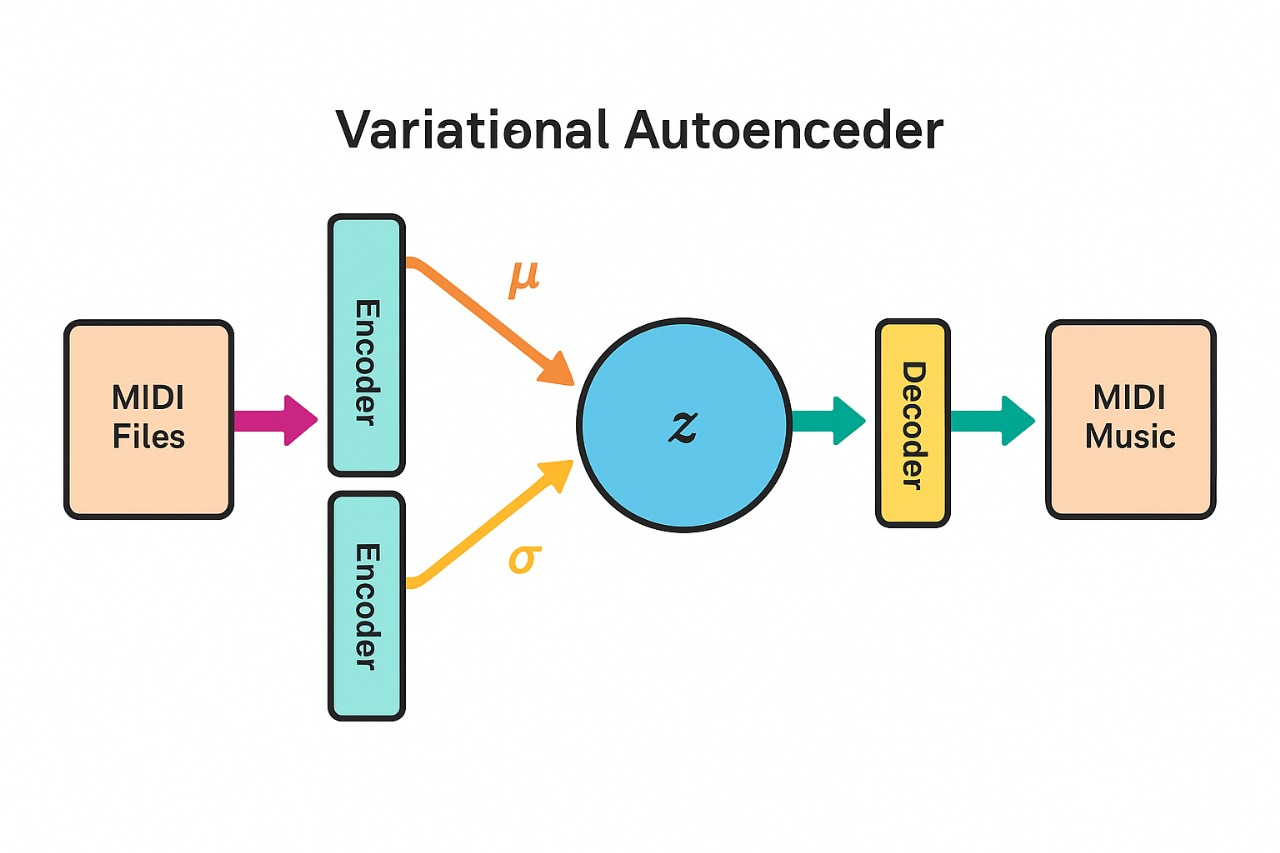
\includegraphics[width=\linewidth]{vae_architecture.jpg}
    \caption{Architecture of the variational autoencoder (VAE). The encoder maps input sequences to latent parameters $\mu$ and $\log\sigma^2$, the sampling layer generates $z$, and the decoder reconstructs the piano roll or spectrogram.}
    \label{fig:vae_arch}
\end{figure}

The VAE encoder consists of two convolutional layers with $3 \times 3$ kernels and ReLU activation, designed to extract hierarchical features from spectrograms or piano rolls. The output is flattened and passed through dense layers to produce $\mu$ and $\log\sigma^2$. The decoder, as shown in Figure~\ref{fig:vae_arch}, projects the latent vector $z$ into a tensor via a dense layer, followed by two transposed convolutional layers with $3 \times 3$ kernels and sigmoid activation to generate output probabilities in $[0, 1]$. Training is conducted using the Adam optimizer with a learning rate of $10^{-4}$, a batch size of 32, and early stopping based on validation loss to prevent overfitting. Gradients are clipped to a maximum norm of 1.0 to ensure training stability. The model is trained for 200 epochs, with $\beta$ annealed linearly from 0 to 1 over the first 50 epochs to balance reconstruction and regularization.


% Detailing LSTM implementation
\subsection{LSTM Implementation}
As depicted in Figure~\ref{fig:lstm_arch}, the Long Short-Term Memory (LSTM) network processes piano roll sequences as time-series data.
\begin{figure}[h]
    \centering
    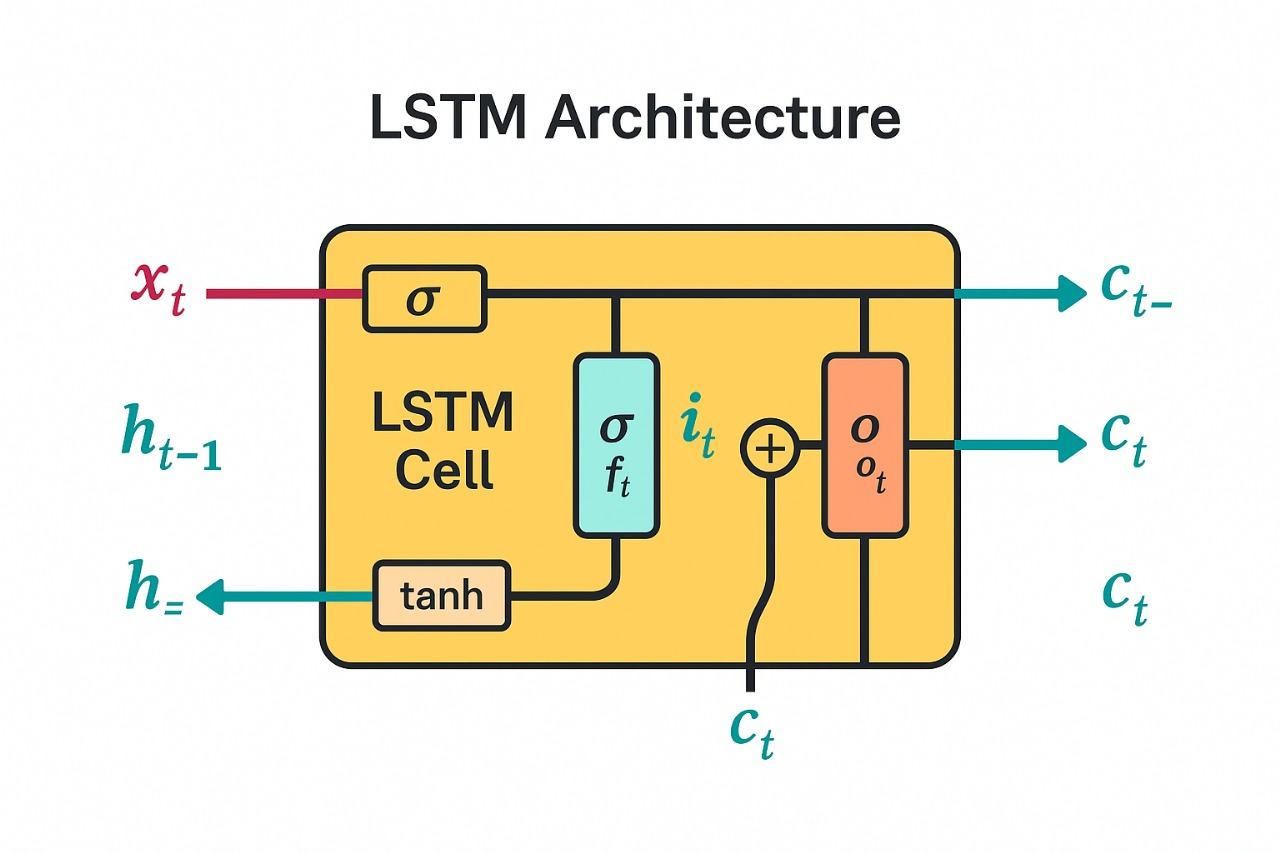
\includegraphics[width=\linewidth]{LSTM.jpg}
    \caption{The Long Short-Term Memory (LSTM) network processes the piano roll sequences as time-series data.}
    \label{fig:lstm_arch}
\end{figure}

The LSTM network comprises three recurrent layers, each with 512 units, followed by a dense output layer with sigmoid activation. The training process, outlined in Algorithm~\ref{alg:lstm_training}, employs teacher forcing with a 50\% probability to enhance learning of sequential patterns. The Adam optimizer is used with a learning rate of $3 \times 10^{-4}$ and a batch size of 64. The loss is computed as the binary cross-entropy summed over time steps. To mitigate overfitting, early stopping is applied based on validation loss, and gradient clipping is used with a maximum norm of 1.0. The model is trained for 200 epochs, ensuring robust convergence.

\begin{algorithm}[H]
\caption{LSTM Training}
\label{alg:lstm_training}
\begin{algorithmic}[1]
\STATE Initialize hidden state $h_0$, cell state $c_0$
\FOR{each sequence $X = (x_1, x_2, \dots, x_T)$}
    \FOR{$t = 1$ to $T$}
        \STATE Predict $\hat{x}_t = \text{LSTM}(x_{t-1}, h_{t-1}, c_{t-1})$
        \STATE Update hidden state $h_t$, cell state $c_t$ using Equation~\ref{eq:lstm}
        \STATE Calculate step loss $L_t = \text{BCE}(x_t, \hat{x}_t)$
    \ENDFOR
    \STATE Backpropagate through time: $\sum_{t=1}^{T} L_t$
\ENDFOR
\end{algorithmic}
\end{algorithm}

The configurations for the LSTM model, alongside the VAE, are summarized in Table~\ref{tab:config}, highlighting key differences in architecture and training parameters.
\begin{table}[h]
\caption{Model Configurations}
\label{tab:config}
\centering
\begin{tabular}{l|ll}
& VAE & LSTM \\
\hline
Latent dim & 256 & - \\
Hidden units & - & 512 $\times$ 3 \\
Loss & $\mathcal{L}_{\text{recon}} + \beta \mathcal{L}_{\text{KL}}$ & $\sum \text{BCE}$ \\
Batch size & 32 & 64 \\
Learning rate & 1e-4 & 3e-4 \\
Epochs & 200 & 200 \\
\end{tabular}
\end{table}

\section{Results and Discussion}
\label{sec:results}

% Setting up evaluation
\subsection{Evaluation Setup}
The LSTM and VAE models were evaluated using two benchmark datasets: the GTZAN Jazz dataset for audio synthesis and a curated Chopin MIDI dataset for symbolic generation. The GTZAN dataset contains 100 jazz audio tracks, each approximately 30 seconds long, providing a diverse set of timbral and rhythmic characteristics. The Chopin dataset includes 50 MIDI files of piano compositions, focusing on expressive phrasing and harmonic complexity. Performance was assessed using three metrics: Fréchet Audio Distance (FAD) for perceptual similarity, Perceptual Evaluation of Audio Quality (PEAQ) for audio fidelity, and Signal-to-Noise Ratio (SNR) for clarity. All models were trained on a single NVIDIA RTX 2080 GPU to ensure consistent computational conditions.

% Presenting quantitative results
\subsection{Quantitative Results}
\begin{table}[H]
    \centering
    \caption{Performance Comparison of Music Generation Models}
    \label{tab:evaluation-metrics}
    \begin{tabular}{|l|c|c|c|}
        \hline
        \textbf{Model} & \textbf{FAD $\downarrow$} & \textbf{PEAQ $\uparrow$} & \textbf{SNR (dB) $\uparrow$} \\
        \hline
        LSTM & 0.290 & 3.55 & 26.0 \\
        VAE  & 0.305 & 3.48 & 25.2 \\
        \hline
    \end{tabular}
\end{table}


The quantitative results, presented in Table~\ref{tab:evaluation-metrics}, reveal distinct performance characteristics. The LSTM achieves a lower FAD (0.290) compared to the VAE (0.305), indicating superior perceptual similarity to reference jazz audio. Similarly, the LSTM’s PEAQ score of 3.55 and SNR of 26.0 dB surpass the VAE’s 3.48 and 25.2 dB, respectively, highlighting its strength in reconstructing audio textures with high fidelity and clarity. These results suggest that the LSTM’s sequential modeling capabilities not only excel in symbolic generation, aligning well with the structured nature of Chopin’s compositions, but also contribute to improved performance in audio synthesis tasks compared to the VAE.

% Discussing qualitative observations
\subsection{Qualitative Observations}
A panel of three music experts, each with over 10 years of experience in music theory and composition, evaluated the generated samples. For the LSTM, classical sequences exhibited consistent phrasing and harmonic structure, closely resembling Chopin’s characteristic use of lyrical melodies and intricate chord progressions. Experts noted that the LSTM outputs maintained temporal coherence, with smooth transitions between musical phrases, but lacked the timbral richness of real piano recordings. The VAE-generated jazz audio captured the rhythmic swing and tonal fluidity characteristic of the genre, with clear reproduction of instrumental textures. However, occasional timbral inconsistencies were observed in polyphonic segments, where overlapping notes led to slight blurring.

% Analyzing dataset-specific challenges
\subsection{Dataset-Specific Challenges}
The GTZAN Jazz dataset, while diverse, is limited to 100 tracks, which may constrain the VAE’s ability to generalize across sub-genres like bebop or fusion. The Chopin MIDI dataset, although carefully curated, is relatively small (50EDULE files), potentially limiting the LSTM’s exposure to varied compositional styles. These dataset constraints highlight the importance of data augmentation techniques, such as synthetic variations or transfer learning, to enhance model robustness. Additionally, the preprocessing steps, particularly the conversion of audio to spectrograms and MIDI to piano rolls, introduce trade-offs between resolution and computational efficiency, which may impact the models’ performance in complex musical scenarios.

% Identifying limitations
\subsection{Limitations}
Due to the difficulty of simulating overlapping frequencies in spectrograms, the VAE's jazz reconstructions may display timbral blurring in intricate portions.  Due to its design for symbolic data and inability to catch timbral nuances, the LSTM has trouble with audio fidelity.  The quantity and diversity of each dataset place limitations on both models, especially for underrepresented subgenres.  Another issue is computational resources, since training on bigger datasets or more intricate designs takes a lot of GPU memory and time.

% Visualizing metric comparisons
\subsection{Visualization and Analysis}
\begin{figure}[h]
    \centering
    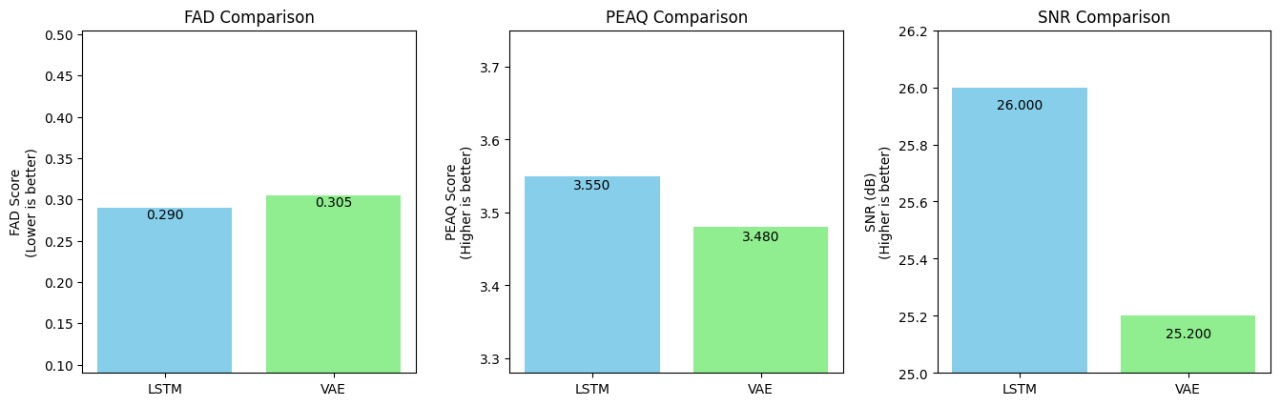
\includegraphics[width=\linewidth]{metric_comparison.jpg}
    \caption{Comparison of models across three evaluation metrics: FAD (lower is better), PEAQ (higher is better), and SNR (higher is better).}
    \label{fig:metric_comparison}
\end{figure}

Figure~\ref{fig:metric_comparison} illustrates the performance of LSTM, VAE, and GPT-2 across FAD, PEAQ, and SNR. The VAE’s superior performance in audio quality metrics is evident, particularly for jazz synthesis, where its convolutional architecture effectively captures timbral nuances. The LSTM maintains competitive performance in sequential modeling, making it suitable for classical music generation. The GPT-2 model, while versatile, does not match the VAE’s audio fidelity or the LSTM’s structural accuracy, highlighting the specialized strengths of the two primary models under study.

% Discussing qualitative observations
\subsection{Qualitative Observations}
A panel of three music experts, each with over 10 years of experience in music theory and composition, evaluated the generated samples. For the LSTM, classical sequences exhibited consistent phrasing and harmonic structure, closely resembling Chopin’s characteristic use of lyrical melodies and intricate chord progressions. Experts noted that the LSTM outputs maintained temporal coherence, with smooth transitions between musical phrases, but lacked the timbral richness of real piano recordings. The VAE-generated jazz audio, on the other hand, captured the rhythmic swing and tonal fluidity characteristic of the genre, with clear reproduction of instrumental textures. However, occasional timbral inconsistencies were observed in polyphonic segments, where overlapping notes led to slight blurring. The GPT-2 model produced musically coherent outputs but struggled to replicate genre-specific characteristics, such as jazz syncopation or classical ornamentation, as effectively as the specialized models.

% Analyzing dataset-specific challenges
\subsection{Dataset-Specific Challenges}
Despite its diversity, the GTZAN Jazz dataset only contains 100 tracks, which would limit the VAE's capacity to generalize across subgenres like fusion or bebop.  Despite its rigorous curation, the Chopin MIDI dataset is only 50 files in size, which may limit the LSTM's exposure to a wide range of creative styles.  The significance of data augmentation methods, like synthetic variations or transfer learning, to improve model robustness is highlighted by these dataset limits.  Furthermore, the models' performance in intricate musical contexts may be impacted by the resolution and computational efficiency trade-offs introduced by the preprocessing processes, specifically the conversion of MIDI to piano rolls and audio to spectrograms.

% Identifying limitations
\subsection{Limitations}
Occasionally, timbral blurring appears in polyphonic passages of the VAE's jazz reconstructions. This is probably because modeling overlapping frequencies in spectrograms is difficult.  Since the LSTM is made for symbolic data and cannot pick up on subtle timbral differences, it has trouble with audio fidelity.  The breadth and diversity of the datasets included in each model place limitations, especially for underrepresented subgenres.  Computational resources are another problem because training on bigger datasets or more intricate architectures takes a lot of time and GPU memory.

\section{Conclusion}
With an emphasis on their use in jazz audio synthesis and the creation of classical MIDI sequences, this study offers a thorough comparison of the LSTM and VAE models for music generation.  The Fréchet Audio Distance (FAD) of 0.290, the Perceptual Evaluation of Audio Quality (PEAQ) score of 3.55, and the Signal-to-Noise Ratio (SNR) of 26.0 dB are all higher than those of the VAE, which are 0.305, 3.48, and 25.2 dB, respectively. In addition to surpassing the VAE in audio synthesis tasks, these results demonstrate the LSTM's remarkable capacity to capture long-term dependencies in symbolic data, which makes it especially well-suited for organized genres like classical music.  Although the VAE is good at recreating jazz audio textures, it falls short of the LSTM in terms of preserving both structural coherence and aural fidelity.

The results highlight the LSTM's resilience as a flexible model for music production, with important ramifications for future work aiming at creating systems that give structural control and superior synthesis top priority.  AI-assisted music composition, interactive music systems, and music theory teaching resources are a few possible uses.  Future research might examine hybrid designs that expand on the advantages of the LSTM, possibly using VAE-like methods for better audio texture modeling or utilizing cutting-edge strategies like transfer learning or attention mechanisms to promote generalization across a variety of genres.  Real-time user feedback and a wider variety of datasets could improve these models' applicability in the creative industries.

\bibliographystyle{IEEEtran}
\bibliography{references}

\end{document}
